%-----------------------------------------------------------------------------%
\chapter{\babLima}
\label{bab:5}
%-----------------------------------------------------------------------------%
Bab ini membahas rangkaian evaluasi untuk menilai keandalan sistem \f{Green} VRPTW, dimulai dari Validasi Akurasi \f{Drive Cycle Generation} (Skenario I) untuk memastikan model \f{machine learning} autoregresif dan Markov Chain mampu mereplikasi profil berkendara, akselerasi, dan beban mesin (VSP) dari data nyata. Selanjutnya, Validasi Akurasi Estimasi Emisi (Skenario II) dilakukan dengan membandingkan hasil perhitungan emisi MOVESTAR terhadap pengukuran langsung menggunakan perangkat IoT. Terakhir, Evaluasi Kinerja Perangkat Keras Sistem IoT meninjau stabilitas sensor dan reliabilitas akuisisi data, sehingga ketiga evaluasi ini secara keseluruhan menunjukkan tingkat akurasi model dan kesiapan sistem untuk mendukung pengambilan keputusan logistik yang lebih berkelanjutan.

%-----------------------------------------------------------------------------%
\section{Validasi Akurasi Estimasi Emisi (Skenario I)}
\label{sec:validasiSkenario1}
%-----------------------------------------------------------------------------%
Validasi ini merupakan tahap kritis untuk membuktikan akurasi metode estimasi profil kecepatan yang dikembangkan. Pengujian dilakukan dengan membandingkan performa dua pendekatan pembangkitan siklus berkendara, yaitu model \f{machine learning} (ML) berbasis autoregresif dan model probabilistik Markov Chain (MCM), terhadap data riil (\f{ground truth}) yang direkam dari kendaraan uji. Tujuan utama validasi adalah menentukan model mana yang paling akurat dalam merepresentasikan karakteristik berkendara nyata, baik dari segi statistik kecepatan (v), dinamika akselerasi (a), hingga distribusi beban mesin (VSP) yang diperoleh dari perhitungan MOVESTAR.

%-----------------------------------------------------------------------------%
\subsection{Analisis Komparatif Performa Algoritma dalam Replikasi Profil Kecepatan}
\label{sec:analisisKomparatif}
%-----------------------------------------------------------------------------%
Pada tahap ini, dilakukan evaluasi terhadap lima algoritma \f{machine learning} untuk menentukan model terbaik yang akan digunakan dalam simulasi \f{Green Routing}. Pengujian dilakukan menggunakan metrik \f{R-squared} ($R^2$), \f{root mean square error} (RMSE), dan \f{mean absolute error} (MAE). Perbandingan ini bertujuan untuk melihat sejauh mana masing-masing arsitektur mampu menangkap kompleksitas non-linear dari dinamika kecepatan kendaraan per detik.

%-----------------------------------------------------------------------------%
\subsubsection{Analisis Algoritma untuk Memprediksi \f{Speed}}
\label{sec:analisisSpeed}
%-----------------------------------------------------------------------------%
\begin{figure}[t!]
    \centering
    \includegraphics[width=0.8\textwidth]{assets/pics/tabel_perbandingan_model.png}
    \caption{Tabel perbandingan metrik evaluasi model ML (Speed)}
    \label{fig:perbandinganModel}
\end{figure}

Model \f{Random Forest} (RF) dalam penelitian ini unggul dengan nilai RMSE terendah (0,4183 m/s) dan $R^2$ tertinggi (0,9805), berakar pada kecocokan arsitektur \f{bootstrap aggregating} (\f{bagging}) dengan karakteristik data pergerakan kendaraan yang fluktuatif. Dengan melatih banyak pohon secara independen dan mengambil rata-ratanya, RF secara alami mampu "menghaluskan" prediksi ekstrem dan memitigasi \f{noise} dari pengereman mendadak atau gangguan sinyal GPS yang sering menyebabkan \f{overfitting} pada \f{Decision Tree} tunggal atau koreksi residu berlebih pada model XGBoost.

Kemampuan RF dalam menangkap interaksi non-linear tingkat tinggi dari 18 fitur multidimensi, termasuk fitur spasial, temporal, dan statistik \f{rolling}, menjadikannya lebih stabil dibandingkan SVR dalam memetakan hubungan kompleks antara geometri jalan dan beban mesin. Selain itu, konsistensi RF pada fitur autoregresif menghasilkan transisi kecepatan yang halus dan logis secara fisik, yang tercermin dalam skor $R^2$ akselerasi turunan sebesar 0,8498. Hal ini sangat krusial bagi model MOVESTAR karena memastikan distribusi VSP Bins tidak bias dan tetap berada dalam koridor fisik yang stabil.

Dalam analisis komparatif, model \f{ensemble} RF menunjukkan stabilitas yang lebih unggul dibandingkan \f{Decision Tree} (DT) yang mencatat skor $R^2$ terendah (0,9699) dan RMSE tertinggi (0,5204 m/s) akibat struktur DT yang kaku dan rentan \f{overfitting} terhadap dinamika data. Meskipun XGBoost memberikan performa kompetitif sesuai riset \cite{rubasinghe2023}, RF tetap memberikan stabilitas yang lebih baik terhadap variasi gaya berkendara individu pada rute BSD-UI.

Apabila dibandingkan dengan SVR yang memiliki $R^2$ stabil sebesar 0,9776, RF menawarkan efisiensi yang lebih tinggi dalam menangani fitur berdimensi tinggi dan juga memiliki waktu komputasi lebih cepat dibanding SVR yang waktu komputasinya sangat sensitif terhadap skala fitur. Sementara itu, meskipun ANN mencatat nilai MAE (0,3077 m/s) dan MAPE (8,10\%) terendah yang menunjukkan akurasi rata-rata sangat baik sesuai temuan \cite{park2011}, nilai RMSE-nya tetap lebih tinggi (0,4958 m/s) daripada RF. Hal ini menegaskan bahwa dalam konteks perhitungan emisi yang sangat sensitif terhadap \f{outliers}, RF lebih efektif dalam memitigasi kesalahan prediksi besar yang dapat mendistorsi nilai VSP, sehingga lebih handal dalam menggeneralisasi "aturan fisik" berkendara pada rute baru.


%-----------------------------------------------------------------------------%
\subsubsection{Analisis Algoritma untuk Memprediksi Akselerasi}
\label{sec:analisisAkselerasi}
%-----------------------------------------------------------------------------%
Untuk menjamin bahwa model tidak hanya akurat secara statistik tetapi juga konsisten secara fisik, dilakukan validasi terhadap akselerasi turunan (\f{derived acceleration}). Hasil menunjukkan bahwa profil kecepatan yang dibangkitkan oleh model terbaik mampu menghasilkan nilai akselerasi dengan skor $R^2$ sebesar 0.8498 dan RMSE 0.2565 $m/s^2$. Capaian ini membuktikan bahwa mekanisme autoregresif yang dikembangkan berhasil menjaga kontinuitas temporal antar-detik, sehingga profil \f{drive cycle} yang dihasilkan tidak memiliki lonjakan kecepatan yang tidak realistis.

\begin{figure}[t!]
    \centering
    \includegraphics[width=1\textwidth]{assets/pics/result_accel_rf.png}
    \caption{Gambar Grafik Perbandingan Hasil Prediksi Akselerasi vs Ground Truth}
    \label{fig:perbandinganModel}
\end{figure}

%-----------------------------------------------------------------------------%
\subsubsection{Penentuan Model Final untuk Sistem \f{Green Routing}}
\label{sec:penentuanModelFinal}
%-----------------------------------------------------------------------------%
Berdasarkan perbandingan metrik pada Gambar \ref{fig:perbandinganModel}, diperoleh beberapa poin diskusi utama untuk menentukan algoritma yang dijadikan model untuk tahap inferensi.

\begin{enumerate}
    \item Analisis Konsistensi Fisik dan Dinamika Kendaraan \\
    Meskipun model ANN menunjukkan nilai MAE dan MAPE yang sedikit lebih rendah (lebih akurat secara rata-rata persentase), model \f{Random Forest} terpilih karena keunggulannya pada nilai $R^2$ (0,9806) dan RMSE (0,4184 m/s). Lebih lanjut, validasi pada \f{derived acceleration} (akselerasi turunan) menghasilkan skor yang cukup baik, $R^2$ sebesar 0,8498 dengan RMSE 0,2565 $m/s^2$. Nilai ini sangat krusial karena membuktikan bahwa model tidak hanya akurat dalam memprediksi angka kecepatan, tetapi juga menjaga konsistensi transisi antar-detik. Kemampuan ini meminimalisir terjadinya "lonjakan" kecepatan yang tidak realistis secara fisik, yang sering terjadi pada model berbasis pohon (\f{tree-based}) tunggal seperti \f{Decision Tree}.

    \item Sensitivitas RMSE terhadap Estimasi Emisi MOVESTAR \\
    
    \begin{figure}[t!]
    \centering
    \includegraphics[width=0.6\textwidth]{assets/pics/hasil_rf.png}
    \caption{Hasil Akurasi Random Forest}
    \label{fig:hasilRF}
    \end{figure}

    Dalam pemodelan emisi mikroskopik, nilai RMSE menjadi parameter evaluasi yang lebih krusial dibandingkan MAE. RMSE yang rendah pada model \f{Random Forest} (setara 1,51 km/h) memberikan jaminan bahwa deviasi prediksi pada titik-titik kritis (seperti akselerasi tajam) tetap terkontrol. Karena perhitungan \f{Vehicle Specific Power} (VSP) dalam MOVESTAR sangat sensitif terhadap nilai akselerasi ($a$), kesalahan kecil pada prediksi kecepatan yang beruntun akan mengakibatkan kesalahan kuadrat pada nilai emisi. Dengan RMSE akselerasi yang hanya sebesar 0,2565 $m/s^2$, model \f{Random Forest} dipastikan dapat menghasilkan distribusi VSP Bins yang stabil, sehingga estimasi polutan \ce{CO2}, HC, dan CO terhindar dari nilai \f{outlier} yang ekstrem.

    \item Kesimpulan Pemilihan Model Final \\
    Berdasarkan analisis di atas, model \f{Random Forest} ditetapkan sebagai model final untuk diimplementasikan ke dalam modul \f{Inference} sistem \f{Green Routing}. Model ini dipilih karena berhasil mencapai keseimbangan optimal antara akurasi statistik (skor $R^2$ tertinggi) dan stabilitas fisik (RMSE terendah). Dengan performa ini, model diharapkan mampu menghasilkan profil \f{drive cycle} sintetis yang paling mendekati karakteristik berkendara riil, yang menjadi prasyarat utama dalam menentukan rute dengan emisi terendah bagi pengguna.
\end{enumerate}

%-----------------------------------------------------------------------------%
\subsection{Hasil Karakteristik Replikasi Profil Kecepatan}
\label{sec:hasilReplikasiKecepatan}
%-----------------------------------------------------------------------------%
Berdasarkan hasil evaluasi performa model \f{machine learning}, \f{Random Forest} (RF) menunjukkan akurasi terbaik dibandingkan algoritma lain, dengan \f{Training} $R^2$ sebesar 0,9806, RMSE 0,4184 m/s ($\approx$1,51 km/jam), dan MAE 0,2795 m/s ($\approx$1,09 km/jam). Nilai ini mengindikasikan kemampuan RF yang sangat baik dalam mereplikasi variasi kecepatan kendaraan secara detik-per-detik dengan kesalahan yang relatif kecil.

Keunggulan \f{Random Forest} pada kasus ini terutama disebabkan oleh kemampuannya dalam menangkap hubungan \f{non-linear} dan interaksi kompleks antar fitur temporal (seperti \f{lag} kecepatan, \f{rolling mean} 5 detik, dan karakteristik segmen jalan) tanpa memerlukan asumsi bentuk fungsi tertentu. \f{Driving cycle} dipengaruhi oleh variasi kecepatan jangka pendek (\f{short-term variations}) dan perubahan kondisi berkendara pada skala mikro, seperti transisi cepat antara akselerasi dan deselerasi. Karakteristik ini menyebabkan pola kecepatan bersifat tidak stabil dan kontekstual, sehingga sulit dimodelkan oleh pendekatan linear.

Selain itu, mekanisme \f{ensemble} berbasis \f{bootstrap aggregation} (\f{bagging}) pada \f{Random Forest} membuat model lebih stabil dan \f{robust} terhadap \f{noise} dibandingkan model tunggal seperti \f{Decision Tree}, serta mengurangi risiko \f{overfitting} yang dapat muncul pada model berkapasitas tinggi seperti ANN atau \f{boosting-based models} pada data yang memiliki korelasi temporal kuat. Berbeda dengan XGBoost, XGBoost membangun pohon secara sekuensial dan cenderung lebih sensitif terhadap \f{error} residual lokal, \f{Random Forest} mampu menghasilkan prediksi yang lebih halus (\f{smooth}) dan konsisten, sehingga lebih sesuai untuk mereplikasi profil kecepatan kontinu pada \f{driving cycle}. Dengan karakteristik tersebut, \f{Random Forest} menjadi model yang paling seimbang antara akurasi, stabilitas, dan kemampuan generalisasi untuk mereplikasi profil kecepatan kendaraan sebagai dasar estimasi beban mesin (VSP) dan emisi secara keseluruhan.

\begin{table}
    \centering
    \caption{Perbandingan Parameter Kinematik (Kecepatan dan Akselerasi)}
    \label{tab:evaluasiAkurasiEmisi}
    \begin{tabular}{|l|l|l|l|}
        \hline
        \bo{Parameter Evaluasi} & \bo{Ground Truth} & \bo{Model ML (Random Forest)} & \bo{Model Markov Chain} \\
        \hline
        Kecepatan Rata-rata & 25,19 km/jam & 24,78 km/jam & 23,20 km/jam \\
        \hline
        Selisih Kecepatan Absolut & - & 0,41 km/jam & 1,99 km/jam \\
        \hline
        Akselerasi Rata-rata & $\sim$0,001 m/s$^2$ & 0,0001 m/s$^2$ & -0,1 m/s$^2$ \\
        \hline
        Selisih Akselerasi Absolut & - & 0,0009 m/s$^2$ & 0,086 m/s$^2$ \\
        \hline
    \end{tabular}
\end{table}

Berdasarkan Tabel \ref{tab:evaluasiAkurasiEmisi}, model \f{machine learning} menunjukkan keunggulan dalam mereplikasi karakteristik profil kecepatan. Model ML mampu memprediksi kecepatan rata-rata dengan deviasi yang sangat minim, yakni hanya selisih 0,41 km/jam dari data asli. Sebaliknya, model Markov Chain memiliki deviasi yang lebih besar (1,99 km/jam), cenderung menghasilkan profil kecepatan yang lebih rendah dari kenyataan.

\begin{figure}[t!]
    \centering
    \includegraphics[width=\textwidth]{assets/pics/compare_speed.png}
    \caption{Prediksi Kecepatan Detik per Detik dengan \f{Machine Learning}}
    \label{fig:prediksiKecepatanML}
\end{figure}

Keunggulan model ML ini mengindikasikan bahwa penggunaan fitur kontekstual, seperti \f{rolling mean} (rata-rata bergerak 5 detik) dan \f{segment average}, sangat efektif menjaga prediksi model agar tetap berada dalam koridor kecepatan yang relevan dengan kondisi jalan spesifik. Sebaliknya, model Markov Chain yang murni berbasis probabilitas transisi antar-\f{state} cenderung kehilangan konteks tren perjalanan jangka panjang. Markov memang bertujuan meniru distribusi statistik, bukan memprediksi nilai eksak pada detik ke-t, sehingga perbandingan langsung \f{point-to-point} menjadi tidak valid.

Selain rata-rata, akurasi prediksi dievaluasi menggunakan metrik \f{root mean square error} (RMSE) untuk kecepatan. Metrik ini mengukur rata-rata besaran kesalahan prediksi model terhadap data aktual pada setiap detiknya. Pendekatan ini memastikan bahwa evaluasi berfokus pada kemampuan model dalam mereplikasi karakteristik beban mesin dan profil energi secara keseluruhan, yang merupakan faktor penentu total emisi, terlepas dari kapan kejadian tersebut terjadi dalam domain waktu. Saat membandingkan ML dan Markov, RMSE hanya disertakan untuk menunjukkan keunggulan tambahan ML (bisa prediksi waktu), bukan sebagai kelemahan Markov.

Meskipun demikian, Markov tetap dinilai valid karena tujuannya memang untuk mereplikasi distribusi statistik, bukan prediksi kecepatan per detik (\f{time alignment}). Performa Markov dalam konteks penelitian ini hanya dievaluasi pada kemiripan bentuk kurva histogram kecepatan, dan bukan pada akurasi temporal. Oleh karena itu, perbandingan antara ML dan Markov difokuskan pada metrik berbasis distribusi karena tujuan penelitian ini ada pada emisi yang dihasilkan secara keseluruhan.

%-----------------------------------------------------------------------------%
\subsection{Analisis Distribusi Kecepatan-Akselerasi (\f{Driving Dynamics})}
\label{sec:analisisDrivingDynamics}
%-----------------------------------------------------------------------------%
Setelah mengevaluasi performa prediksi kecepatan pada domain waktu, tahap berikutnya adalah membandingkan kemampuan kedua model, Markov Chain Model (MCM) dan \f{machine learning} autoregresif (ML-AR), dalam mereplikasi karakteristik statistik dari data riil. Validasi perlu dilakukan pada domain frekuensi untuk melihat apakah model mampu mereplikasi pola kombinasi kecepatan dan akselerasi (\f{driving dynamics}) yang terjadi di dunia nyata.

Evaluasi ini berfokus pada tiga variabel utama pembentuk emisi, yaitu kecepatan (v), akselerasi (a), dan \f{Vehicle Specific Power} (VSP). Pendekatan berbasis distribusi ini dipilih karena relevan dengan tujuan akhir penelitian, yaitu mengestimasi total emisi. Dalam perhitungan MOVESTAR, estimasi total emisi sangat bergantung pada frekuensi kemunculan kondisi beban mesin dalam bentuk VSP bin. Dengan demikian, akurasi temporal tidak menjadi prioritas, melainkan kemampuan model untuk menghasilkan distribusi energi kendaraan yang setara dengan data \f{ground truth}.

%-----------------------------------------------------------------------------%
\subsubsection{Analisis Distribusi Kecepatan}
\label{sec:analisisDistribusiKecepatan}
%-----------------------------------------------------------------------------%
\begin{figure}[t!]
    \centering
    \includegraphics[width=0.4\textwidth]{assets/pics/distribusi_kecepatan_mcm.png}
    \caption{Gambar Distribusi Kecepatan dari Pendekatan MCM}
    \label{fig:distribusiKecepatanMCM}
\end{figure}

\begin{figure}[t!]
    \centering
    \includegraphics[width=0.4\textwidth]{assets/pics/distribusi_kecepatan_ml.png}
    \caption{Gambar Distribusi Kecepatan dari Pendekatan ML}
    \label{fig:distribusiKecepatanML}
\end{figure} 

Gambar \ref{fig:distribusiKecepatanMCM} menunjukkan distribusi kecepatan antara data riil dan data sintetis yang dihasilkan oleh model Markov Chain dan gambar \ref{fig:distribusiKecepatanML} menunjukkan distribusi kecepatan yang dihasilkan oleh model \f{machine learning} (ML). Kedua model mampu mereplikasi pola dasar distribusi kecepatan kendaraan, tetapi tingkat kedekatannya dengan data riil berbeda cukup signifikan.

Pada model Markov Chain, kurva kecepatan sintetis tampak mengikuti bentuk umum histogram kecepatan riil, namun terdapat pergeseran distribusi ke arah kecepatan yang lebih rendah. Pola ini tampak dari proporsi frekuensi yang lebih besar pada rentang 0--20 km/jam dibandingkan data riil. Perbedaan ini konsisten dengan hasil statistik, di mana rata-rata kecepatan sintetis Markov (23,20 km/jam) berada 1,99 km/jam lebih rendah dibandingkan rata-rata riil (25,19 km/jam). Fenomena ini merupakan karakteristik umum model Markov, karena mekanisme transisi probabilitas cenderung mempertahankan status kecepatan rendah lebih lama ketika tidak ada konteks dinamika perjalanan yang digunakan sebagai referensi. Dengan kata lain, Markov dapat meniru distribusi global tetapi tidak mampu menangkap pola momentum dan akselerasi berkelanjutan yang terjadi pada situasi berkendara nyata.

Sebaliknya, model \f{machine learning} autoregresif menunjukkan kecocokan distribusi yang jauh lebih baik dengan data riil. Kurva sintetis ML hampir sepenuhnya menumpuk pada histogram kecepatan riil, terutama pada rentang kecepatan 10--40 km/jam yang merupakan wilayah dominan dalam data. Selisih rata-rata kecepatan antara ML dan data riil juga sangat kecil, yaitu hanya 0,41 km/jam, menandakan bahwa model ML tidak hanya meniru bentuk distribusi tetapi juga mempertahankan pusat massa (\f{mean}) distribusi tersebut dengan akurat. Konsistensi ini tercermin dari grafik, di mana puncak distribusi, kemiringan kurva, dan pola penurunan frekuensi pada kecepatan tinggi menunjukkan kesamaan yang baik. Meskipun terdapat sedikit deviasi pada kecepatan di atas 40 km/jam, penyimpangan tersebut tidak mengubah karakteristik distribusi secara keseluruhan.

Kemampuan ML menangkap distribusi kecepatan dengan lebih akurat juga sejalan dengan performa temporalnya yang tinggi ($R^2 = 0,9806$). Hal ini menunjukkan bahwa model ML bukan hanya menjaga kesesuaian bentuk distribusi statistik, tetapi juga mampu mengikuti dinamika perubahan kecepatan dari waktu ke waktu. Dengan demikian, pola berkendara yang dihasilkan menjadi lebih realistis karena model dapat merepresentasikan momentum kendaraan, transisi kecepatan yang cepat, serta variasi akselerasi yang terjadi secara alami pada kondisi lalu lintas sebenarnya. Karakteristik ML (Random Forest) yang sedikit lebih "agresif", untuk mereproduksi perubahan kecepatan yang lebih tajam dibanding model Markov, justru menjadi keunggulan dalam konteks estimasi emisi karena mencegah terjadinya \f{over smoothing} yang berlebihan.

Sebaliknya, Markov cenderung menghasilkan profil kecepatan yang lebih "rata" dan kurang menangkap kejadian-kejadian kritis seperti akselerasi singkat atau perlambatan mendadak. Hal ini terjadi karena mekanisme transisi probabilistik Markov secara alami merata-ratakan peluang antar-\f{state}, sehingga variasi ekstrem atau perubahan mendadak dalam data asli sering kali tereduksi atau bahkan hilang. Padahal, kejadian-kejadian tersebut memiliki kontribusi besar terhadap lonjakan energi kendaraan dan peningkatan emisi sesaat. Oleh karena itu, meskipun Markov valid sebagai model distribusi statistik, ML memberikan representasi dinamika berkendara yang lebih lengkap dan lebih relevan untuk perhitungan emisi berbasis VSP.

%-----------------------------------------------------------------------------%
\subsubsection{Analisis Distribusi Akselerasi}
\label{sec:analisisDistribusiAkselerasi}
%-----------------------------------------------------------------------------%
Evaluasi terhadap akselerasi dilakukan dengan membandingkan nilai rata-rata (\f{mean}) dan besaran kesalahan prediksi akselerasi antara model \f{machine learning} autoregresif (ML-AR) dan model Markov Chain (MCM). Akselerasi menjadi variabel penting dalam perhitungan \f{Vehicle Specific Power} (VSP), meskipun sensitivitasnya terhadap emisi lebih rendah dibanding kecepatan.

\begin{enumerate}
    \item Model \f{machine learning} (ML) \\
    Model ML menunjukkan kemampuan yang baik dalam mempertahankan nilai akselerasi rata-rata yang mendekati data riil. Akselerasi rata-rata pada data riil adalah 0,00014 m/s\textsuperscript{2}, sedangkan akselerasi sintetis ML berada pada 0,00107 m/s\textsuperscript{2}, dengan selisih yang sangat kecil yaitu 0,00093 m/s\textsuperscript{2}. Selisih ini menunjukkan bahwa ML tidak menyebabkan \f{drift} atau bias sistematis terhadap percepatan maupun perlambatan kendaraan. Nilai \f{mean} akselerasi yang hampir nol pada kedua dataset juga menggambarkan bahwa model ML mampu menjaga keseimbangan antara fase akselerasi dan deselerasi seperti pada pola berkendara nyata.
    
    Meskipun demikian, akurasi temporal akselerasi ML (\f{accel} $R^2 = 0,218$) relatif rendah. Hal ini umum terjadi pada model autoregresif karena akselerasi merupakan turunan pertama dari kecepatan dan sangat sensitif terhadap fluktuasi kecil. Walaupun nilai $R^2$ rendah, metrik ini tidak secara langsung memengaruhi kualitas estimasi emisi karena model emisi MOVESTAR menggunakan bin VSP, bukan nilai akselerasi detik-per-detik. Selama kecenderungan akselerasi tidak bias dan rentang nilainya realistis, model tetap valid. Konsistensi ini tercermin dari \f{error} akselerasi yang moderat (RMSE = 0,3219 m/s\textsuperscript{2} dan MAE = 0,2357 m/s\textsuperscript{2}), yang masih berada dalam rentang operasional kendaraan perkotaan.
    
    \item Model Markov Chain \\
    Model Markov Chain menghasilkan profil akselerasi yang lebih fluktuatif dan bias dibandingkan model \f{machine learning}. Berdasarkan Tabel \ref{tab:evaluasiAkurasiEmisi}, rata-rata akselerasi sintetis dari model Markov berada pada sekitar $-0,01$ m/s$^2$, sementara data \f{ground truth} menunjukkan nilai rata-rata yang mendekati nol ($\approx 0$ m/s$^2$), yang merepresentasikan keseimbangan antara fase akselerasi dan deselerasi sepanjang perjalanan. Selisih rata-rata akselerasi sebesar 0,086 m/s$^2$ menunjukkan adanya pergeseran kecenderungan Markov ke arah perlambatan (deselerasi).

    Bias ini muncul secara inheren dari karakteristik model Markov Chain yang hanya mengandalkan probabilitas transisi antar \f{state} kecepatan, tanpa mempertimbangkan dinamika fisik kendaraan seperti kontinuitas gaya dorong, resistansi jalan, maupun respons mesin terhadap perubahan kecepatan. Akibatnya, variasi akselerasi yang dihasilkan menjadi kurang representatif terhadap kondisi riil, dengan rentang akselerasi yang relatif lebih “halus” dan tidak mampu mereplikasi perubahan akselerasi tajam yang umum terjadi pada data aktual.
\end{enumerate}

Perbedaan performa akselerasi antara ML dan Markov tidak berdampak signifikan terhadap kesalahan emisi, selama pola umum akselerasi tetap konsisten dan tidak menghasilkan \f{drift}. Dapat disimpulkan bahwa ML dinilai lebih baik, karena \f{mean} akselerasinya hampir identik dengan data riil dan tidak menunjukkan bias sistematis.

%-----------------------------------------------------------------------------%
\subsubsection{Analisis Distribusi \f{Vehicle Specific Power} (VSP)}
\label{sec:analisisDistribusiVSP}
%-----------------------------------------------------------------------------%
Distribusi \f{Vehicle Specific Power} (VSP) merupakan aspek evaluasi yang paling penting dalam validasi model pembangkitan siklus berkendara karena VSP berfungsi sebagai indikator langsung beban mesin yang mencerminkan kebutuhan daya kendaraan pada setiap detik perjalanan. VSP menggabungkan komponen kecepatan, akselerasi, gaya resistansi aerodinamis, dan gradien jalan ke dalam satu metrik energi yang terstandardisasi, sehingga mampu menangkap kondisi operasional kendaraan secara fisik dan konsisten.

Studi-studi terbaru menunjukkan bahwa VSP merupakan prediktor yang kuat terhadap variasi emisi kendaraan modern. Sebagai contoh, penelitian Gao et al. (2023) menunjukkan bahwa VSP mampu menjelaskan proporsi terbesar variasi emisi \ce{CO2}, CO, dan $NO_x$ dibandingkan variabel kecepatan atau akselerasi secara individual, sehingga pendekatan berbasis VSP \f{bins} tetap unggul untuk estimasi emisi makroskopik. Temuan serupa diperkuat oleh Adeeb et al. (2025) yang menggunakan teknik \f{unsupervised learning} untuk memodelkan emisi berdasarkan klaster VSP dan menunjukkan bahwa transisi antar-rentang VSP berkorelasi langsung dengan lonjakan emisi sesaat pada kondisi akselerasi tinggi. Selain itu, penelitian Wang et al. (2020) menunjukkan bahwa meskipun terdapat variasi kecil dalam emisi pada VSP yang sama, distribusi frekuensi VSP tetap merupakan representasi terbaik dari beban mesin untuk model-model inventarisasi emisi.

\begin{figure}[t!]
    \centering
    \includegraphics[width=0.4\textwidth]{assets/pics/distribusi_vsp_mcm.png}
    \caption{Gambar Distribusi VSP pada pendekatan Markov Chain}
    \label{fig:distribusiVSPMCM}
\end{figure}

\begin{figure}[t!]
    \centering
    \includegraphics[width=0.4\textwidth]{assets/pics/distribusi_vsp_ml.png}
    \caption{Gambar Distribusi VSP pada pendekatan ML}
    \label{fig:distribusiVSPML}
\end{figure}

Dengan dasar tersebut, kesesuaian distribusi VSP antara data sintetis dan data riil menjadi indikator paling penting dalam menilai apakah model \f{drive cycle} dapat menghasilkan estimasi emisi yang akurat. Hasil validasi menunjukkan bahwa model Markov Chain mampu mereplikasi pola dasar distribusi VSP dengan baik, ditunjukkan oleh nilai RMSE distribusi sebesar 0,027. Grafik memperlihatkan bahwa bentuk kurva sintetis Markov mengikuti pola riil, terutama pada area puncak distribusi (sekitar -2 hingga 2 kW/ton). Meskipun terdapat sedikit \f{overrepresentation} pada rentang VSP rendah (-5 hingga 0 kW/ton), penyimpangan ini masih berada dalam batas toleransi untuk estimasi emisi agregat karena bentuk kurva secara keseluruhan tetap terpelihara.

Di sisi lain, model \f{machine learning} autoregresif menunjukkan kesesuaian yang jauh lebih tinggi, dengan nilai RMSE distribusi hanya 0,016, hampir setengah dari nilai Markov. Kurva distribusi ML tampak hampir sepenuhnya tumpang tindih dengan distribusi riil, terutama pada rentang 0--5 kW/ton yang merupakan kondisi beban dominan pada siklus perkotaan. Hal ini menunjukkan bahwa ML tidak hanya mampu meniru bentuk distribusi, tetapi juga menangkap dinamika energi kendaraan secara fisik, menghasilkan profil beban mesin yang jauh lebih mendekati kondisi aktual.

Dalam kasus ini, Markov tetap diterima meskipun variabilitasnya lebih besar karena distribusi VSP yang dihasilkan tetap berada dalam batas toleransi validasi (RMSE VSP = 0,0369). Secara keseluruhan, hasil ini menunjukkan bahwa kedua model lolos validasi distribusi VSP, tetapi ML memberikan akurasi yang jauh lebih tinggi dan sangat sesuai untuk estimasi emisi berbasis frekuensi bin. Dengan demikian, model ML direkomendasikan sebagai pendekatan utama dalam pembangkitan siklus berkendara pada penelitian ini, terutama jika diperlukan estimasi emisi yang lebih presisi dan sensitif terhadap variasi energi kendaraan.

%-----------------------------------------------------------------------------%
\subsubsection{Implikasi Perbedaan Akurasi VSP terhadap Estimasi Emisi}
\label{sec:implikasiAkurasiVSP}
%-----------------------------------------------------------------------------%
Perbedaan RMSE antara Markov dan ML berdampak langsung pada kualitas estimasi emisi. Karena setiap bin VSP dalam MOVESTAR memiliki faktor emisi yang berbeda---misalnya emisi \ce{CO2} lebih tinggi pada bin beban besar (VSP $>$ 10) dan lebih rendah pada kondisi \f{coasting} (VSP $<$ 0)---maka kesalahan distribusi pada salah satu rentang dapat mempengaruhi total emisi secara proporsional.

\begin{enumerate}
    \item ML menghasilkan estimasi emisi yang lebih stabil dan mendekati kondisi nyata, karena distribusi VSP-nya nyaris identik dengan data riil. Tidak hanya itu, estimasi VSP secara detik per detik pun cukup mendekati \f{ground truth}.
    \begin{figure}[t!]
    \centering
    \includegraphics[width=\textwidth]{assets/pics/compare_vsp.png}
    \caption{Prediksi VSP Detik per Detik dengan \f{Machine Learning}}
    \label{fig:prediksiKecepatanML}
\end{figure}
    \item Markov tetap valid untuk estimasi emisi makroskopik, khususnya pada studi jangka panjang atau inventarisasi emisi yang tidak memerlukan akurasi temporal tinggi. Namun, pada skenario yang membutuhkan evaluasi skala detik atau simulasi respons kendaraan terhadap kondisi jalan spesifik, ML menjadi model yang jauh lebih akurat.
\end{enumerate}

Dengan demikian, evaluasi ini menegaskan bahwa meskipun kedua model memenuhi syarat validasi distribusi VSP, ML-AR merupakan pilihan terbaik ketika penelitian membutuhkan representasi fisik beban mesin yang paling mendekati realitas.

%-----------------------------------------------------------------------------%
\section{Validasi Akurasi Estimasi Emisi (Skenario II)}
\label{sec:validasiSkenario2}
%-----------------------------------------------------------------------------%
Validasi ini bertujuan untuk menguji keandalan model MOVESTAR sebagai dasar perhitungan biaya lingkungan dalam sistem \f{Green} VRPTW. Pengujian dilakukan dengan membandingkan estimasi emisi model terhadap data \f{ground truth} yang direkam oleh sensor IoT pada skenario berkendara nyata (\f{real-world driving}). Fokus utama evaluasi adalah pada dua aspek: (1) kemampuan model menangkap dinamika emisi akibat perubahan perilaku berkendara, dan (2) akurasi estimasi total emisi perjalanan yang menjadi parameter kunci dalam optimasi rute.

%-----------------------------------------------------------------------------%
\subsection{Metodologi Pemrosesan dan Penyelarasan Data}
\label{sec:metodologiPemrosesanData}
%-----------------------------------------------------------------------------%
Sebelum melakukan analisis komparatif, data mentah dari sensor IoT melalui serangkaian proses pra-pemrosesan untuk memastikan integritas dan keselarasan temporal dengan data prediksi model.

Tahap pertama adalah pembersihan data. Data mentah sensor seringkali mengandung \f{noise} dan duplikasi \f{timestamp}. Proses ini meliputi penghapusan data \f{error} (kode -1) dan agregasi data per detik menggunakan rata-rata (\f{mean}) untuk menghasilkan linimasa yang kontinu dan unik (1 Hz).

Tahap selanjutnya adalah konversi satuan. Sensor merekam data dalam satuan konsentrasi (ppm), sedangkan MOVESTAR menghasilkan keluaran massa (gram). Konversi dilakukan menggunakan Hukum Gas Ideal standar (Volume Molar pada 25$^\circ$C dan Massa Molar \ce{CO2} 44,01 g/mol) serta asumsi laju aliran udara konstan sebesar 0,1 L/s yang dihasilkan oleh \f{blower} alat validasi.

Tahap terakhir adalah sinkronisasi waktu. Tantangan utama adalah menentukan titik awal siklus berkendara pada data sensor yang direkam secara kontinu. Digunakan teknik \f{Cross-Correlation Sliding Window} untuk menggeser data sensor terhadap profil prediksi MOVESTAR. Algoritma ini secara otomatis menemukan titik korelasi tertinggi pada indeks waktu 17:20:16, yang kemudian ditetapkan sebagai titik awal sinkronisasi untuk perbandingan \f{side-by-side}.

%-----------------------------------------------------------------------------%
\subsection{Analisis Tren Dinamika Emisi}
\label{sec:analisisTrenDinamika}
%-----------------------------------------------------------------------------%
Evaluasi visual dilakukan dengan membandingkan grafik \f{time-series} emisi per detik antara prediksi model dan hasil pengukuran sensor.

\begin{figure}[t!]
    \centering
    \includegraphics[width=\textwidth]{assets/pics/dinamika_emisi_movestar_vs_sensor.png}
    \caption{Perbandingan Dinamika Emisi per Detik (MOVESTAR vs Sensor IoT)}
    \label{fig:dinamikaEmisi}
\end{figure}

Berdasarkan Gambar \ref{fig:dinamikaEmisi}, terlihat perbedaan karakteristik respons yang jelas antara model komputasi dan sensor fisik:
\begin{itemize}
    \item Responsivitas: Model MOVESTAR (Garis Biru) menunjukkan respons instan terhadap akselerasi kendaraan, menghasilkan lonjakan (\f{spikes}) emisi yang tajam dan tinggi. Hal ini wajar karena model menghitung emisi secara teoritis berdasarkan beban mesin saat itu juga tanpa memperhitungkan keterlambatan fluida.
    \item Efek Peredaman Fisik: Sebaliknya, data sensor (Garis Oranye) menunjukkan grafik yang lebih landai dan teredam. Fenomena ini disebabkan oleh keterbatasan fisik alat ukur, seperti waktu tempuh gas dari mesin ke \f{chamber} dan waktu respons sensor yang tidak seketika, sehingga fluktuasi ekstrem teredam (\f{damped}).
    \item Konsistensi Pola: Meskipun magnitudo (amplitudo) berbeda dan sinkronisasi waktu tidak sempurna, pola naik-turun emisi kedua grafik menunjukkan keselarasan tren. Ketika model memprediksi kenaikan emisi akibat akselerasi, sensor cenderung merekam kenaikan serupa. Hal ini dikonfirmasi oleh nilai korelasi Pearson positif ($r = 0,32$). Meskipun secara statistik nilai ini tergolong lemah akibat adanya \f{time-lag} dan perbedaan responsivitas, korelasi positif ini mengindikasikan bahwa MOVESTAR memiliki kecenderungan arah yang selaras dengan emisi aktual saat terjadi perubahan beban mesin.
\end{itemize}

%-----------------------------------------------------------------------------%
\subsection{Evaluasi Kuantitatif dan Total Emisi}
\label{sec:evaluasiKuantitatif}
%-----------------------------------------------------------------------------%
Dalam konteks algoritma \f{routing}, akurasi total emisi perjalanan (\f{cumulative emission}) jauh lebih kritikal dibandingkan presisi detik-per-detik. Tabel berikut merangkum performa model berdasarkan metrik statistik utama.

\begin{table}
    \centering
    \caption{Ringkasan Metrik Evaluasi Akurasi Emisi}
    \label{tab:ringkasanEvaluasiEmisi}
    \begin{tabular}{|l|l|p{0.4\textwidth}|}
        \hline
        \centering \bo{Metrik Evaluasi} & \centering \bo{Nilai} & \centering \bo{Interpretasi} \tabularnewline
        \hline
        Total Emisi MOVESTAR & 170,09 gram & Prediksi akumulasi emisi untuk satu perjalanan penuh. \\
        \hline
        Total Emisi Sensor & 136,07 gram & Akumulasi pengukuran sensor IoT yang telah dikonversi. \\
        \hline
        Relative Error Total & 25,13 \% & Persentase selisih total emisi antara model dan sensor. \\
        \hline
        RMSE & 1,65 g/s & Rata-rata kesalahan prediksi per detik. \\
        \hline
        Pearson Correlation (r) & 0,32 & Korelasi positif lemah antara prediksi dan observasi. \\
        \hline
    \end{tabular}
\end{table}

Analisis mendalam terhadap hasil tersebut adalah sebagai berikut:

\begin{enumerate}
    \item Sifat Konservatif Model (\f{overestimation}): Terdapat selisih (\f{gap error}) sebesar $\sim$25\% di mana prediksi MOVESTAR secara konsisten lebih tinggi dibandingkan bacaan sensor. Bias ini merupakan hasil yang dapat dijelaskan secara teknis. Koefisien emisi dasar pada model MOVESTAR diturunkan dari basis data \f{US EPA MOVES}, di mana kategori sepeda motor umumnya merepresentasikan kendaraan dengan kapasitas mesin besar ($>250$cc) yang lazim di Amerika Serikat. Sebaliknya, kendaraan uji yang digunakan dalam penelitian ini adalah Yamaha NMAX dengan kapasitas mesin 155cc yang secara inheren jauh lebih efisien bahan bakar. Oleh karena itu, wajar jika emisi aktual yang dihasilkan lebih rendah daripada prediksi model standar. Dalam konteks sistem \f{Green VRPTW}, bias konservatif ini memberikan estimasi batas atas (\f{upper bound}) yang aman untuk perencanaan dampak lingkungan.
    \item Validitas untuk \f{Routing}: Meskipun korelasi detik-ke-detik terbatas ($r=0,32$) yang tercermin pada RMSE, kesalahan ini cenderung bersifat sistematis dan searah. Grafik kumulatif (Subplot 2 pada visualisasi) menunjukkan bahwa akumulasi \f{error} berjalan linier. Hal ini mengimplikasikan bahwa model tetap dapat diandalkan untuk membedakan rute yang "mahal" dan "murah" secara emisi dalam perbandingan relatif.
\end{enumerate}

%-----------------------------------------------------------------------------%
\subsection{Kesimpulan Validasi}
\label{sec:kesimpulanValidasi}
%-----------------------------------------------------------------------------%
Hasil pengujian menyimpulkan bahwa meskipun akurasi temporal pada skala mikro (detik) terbatas akibat kendala fisik sensor, model MOVESTAR cukup memadai digunakan sebagai estimator emisi makroskopis untuk sistem \f{Green} VRPTW. Kemampuannya dalam menangkap tren perilaku berkendara dan sifat estimasinya yang konservatif memberikan landasan yang logis bagi algoritma optimasi untuk membedakan rute yang ramah lingkungan dari rute yang boros emisi secara komparatif.

%-----------------------------------------------------------------------------%
\section{Evaluasi Kinerja Perangkat Keras Sistem IoT}
\label{sec:evaluasiKinerjaIoT}
%-----------------------------------------------------------------------------%
Implementasi perangkat keras sistem IoT pada penelitian ini difokuskan pada integrasi fisik terhadap kendaraan uji untuk memastikan validitas proses akuisisi data dalam kondisi operasional yang dinamis. Pada bagian ini, evaluasi mencakup pada aspek manajemen daya dan durabilitas baterai, analisis responsivitas sensor, integritas daya yang tersimpan di SD Card, dan stabilitas performa sistem IoT pada kondisi dengan kondisi lingkungan bertemperatur yang relatif tinggi dan memiliki getaran yang tinggi.

Tujuan evaluasi kinerja sistem perangkat keras IoT adalah memverifikasi bahwa perangkat keras sistem IoT yang dikembangkan mampu beroperasi secara mandiri dan menghasilkan \f{dataset} yang dapat dipertanggungjawabkan dan digunakan sebagai \f{ground truth} untuk validasi model emisi. Evaluasi dilakukan dengan cara melihat hasil pembacaan sistem IoT yang tersimpan sebagai \f{file csv} (\f{comma-separated values}) dalam SD Card.

%-----------------------------------------------------------------------------%
\subsection{Evaluasi Manajemen Daya dan Durabilitas Baterai}
\label{sec:evaluasiDaya}
%-----------------------------------------------------------------------------%
Berdasarkan analisis \f{log} data yang didapat dari pengujian lapangan, sistem manajemen daya terbukti dapat mendukung operasional dengan durasi panjang. Data rekaman hasil pengujian pada tanggal 13 November 2025 menunjukkan sistem IoT mampu beroperasi secara kontinu selama 1 jam di mana untuk pertama kalinya, sistem IoT beroperasi pada pukul 15:44:55 dan berakhir pada 17:04:24 berdasarkan waktu sistem IoT dengan menggunakan modul RTC tanpa ada interupsi.

\begin{figure}[t!]
    \centering
    \includegraphics[width=\textwidth]{assets/pics/tangkapan_layar_pengujian.png}
    \caption{Tangkapan Layar Permulaan dan Akhir dari Pengujian Pada Tanggal 13 November 2025}
    \label{fig:tangkapanLayarPengujian}
\end{figure}

Selama pengetesan berlangsung, tidak ditemukan indikasi bahwa sistem IoT mengalami \f{restart} jika dilihat dari \f{timestamp} yang terus berjalan secara kronologis sehingga dapat dikonfirmasi bahwa konfigurasi catu daya yang diimplementasi menggunakan baterai 12.000 mAh dengan regulator tegangan pada sistem IoT berhasil menyuplai daya stabil ke seluruh komponen termasuk sensor, mikrokontroler, dan kipas dengan spesifikasinya masing-masing meskipun dalam kondisi beban penuh.

%-----------------------------------------------------------------------------%
\subsection{Analisis Responsivitas Sensor}
\label{sec:analisisResponsivitas}
%-----------------------------------------------------------------------------%
Sensor gas yang digunakan berhasil menampilkan karakteristik respons yang dinamis dengan waktu respons yang cepat dan berhasil memenuhi persyaratan untuk mengembalikan nilai hasil pembacaan sensor pada interval 1 hz di mana pembacaan sensor terbukti dapat disediakan sekali setiap detiknya. Selain itu, dapat diobservasi bahwa sensor analog yang digunakan (MQ-2 dan MQ-7) mampu mengembalikan nilai berupa desimal hingga 2 angka di belakang koma. Dapat dilihat juga untuk sensor \ce{CO2} yang beroperasi secara digital memiliki rentang dinamis yang lebar bahkan hingga di atas 6000 ppm dalam rentang waktu yang singkat yang dapat dilihat pada Gambar \ref{fig:tangkapanLayarPengujian}.

%-----------------------------------------------------------------------------%
\subsection{Integritas Data}
\label{sec:integritasData}
%-----------------------------------------------------------------------------%
Data-data hasil pembacaan sensor juga terbukti dapat tersimpan dengan baik pada SD Card dengan format yang konsisten jika dilihat dari Gambar \ref{fig:tangkapanLayarPengujian}. secara utuh dan memiliki konsistensi \f{sampling} yang terjaga secara temporal tanpa ada data yang kesenggangan antar satu satuan waktu.

%-----------------------------------------------------------------------------%
\subsection{Stabilitas Termal dan Mekanikal}
\label{sec:stabilitasTermal}
%-----------------------------------------------------------------------------%
Dengan solusi desain perangkat keras sistem IoT yang telah dikembangkan, integrasi antara modul Unit Kontrol Utama dengan \f{Mixing Chamber} yang disatukan dengan menggunakan \f{silicone double-sided tape} berhasil bertahan dan utuh bahkan hingga proses pengujian selesai dengan tidak adanya indikasi degradasi kualitas rekatan antara keduanya.

Namun selama proses pengujian, terjadi insiden berupa sistem IoT tidak kuat merekat pada bagian sepatbor sepeda motor kendaraan uji karena luas permukaan yang tidak begitu besar karena bentuk sepatbor yang beragam. Selain itu, biasanya sistem IoT juga kemudian diketahui tidak bisa merekat dengan baik dengan sepatbor kendaraan uji apabila antara \f{silicone double-sided tape} atau sepatbor dalam kondisi basah atau lembab. Jika sistem IoT sudah berhasil direkatkan dengan sepatbor kendaraan uji, sistem IoT dapat bertahan dengan sangat baik sekalipun kendaraan dipacu dalam akselerasi tinggi dan menghantam jalanan yang tidak rata.

Selama proses pengujian sistem IoT dan pengambilan data, sistem IoT dapat berjalan secara optimal tanpa adanya gangguan stabilitas sistem yang terjadi akibat suhu lingkungan. Hal tersebut dibuktikan dari hasil pengujian suhu sistem IoT sebagaimana yang menghasilkan data sebagai berikut.

\begin{figure}[t!]
    \centering
    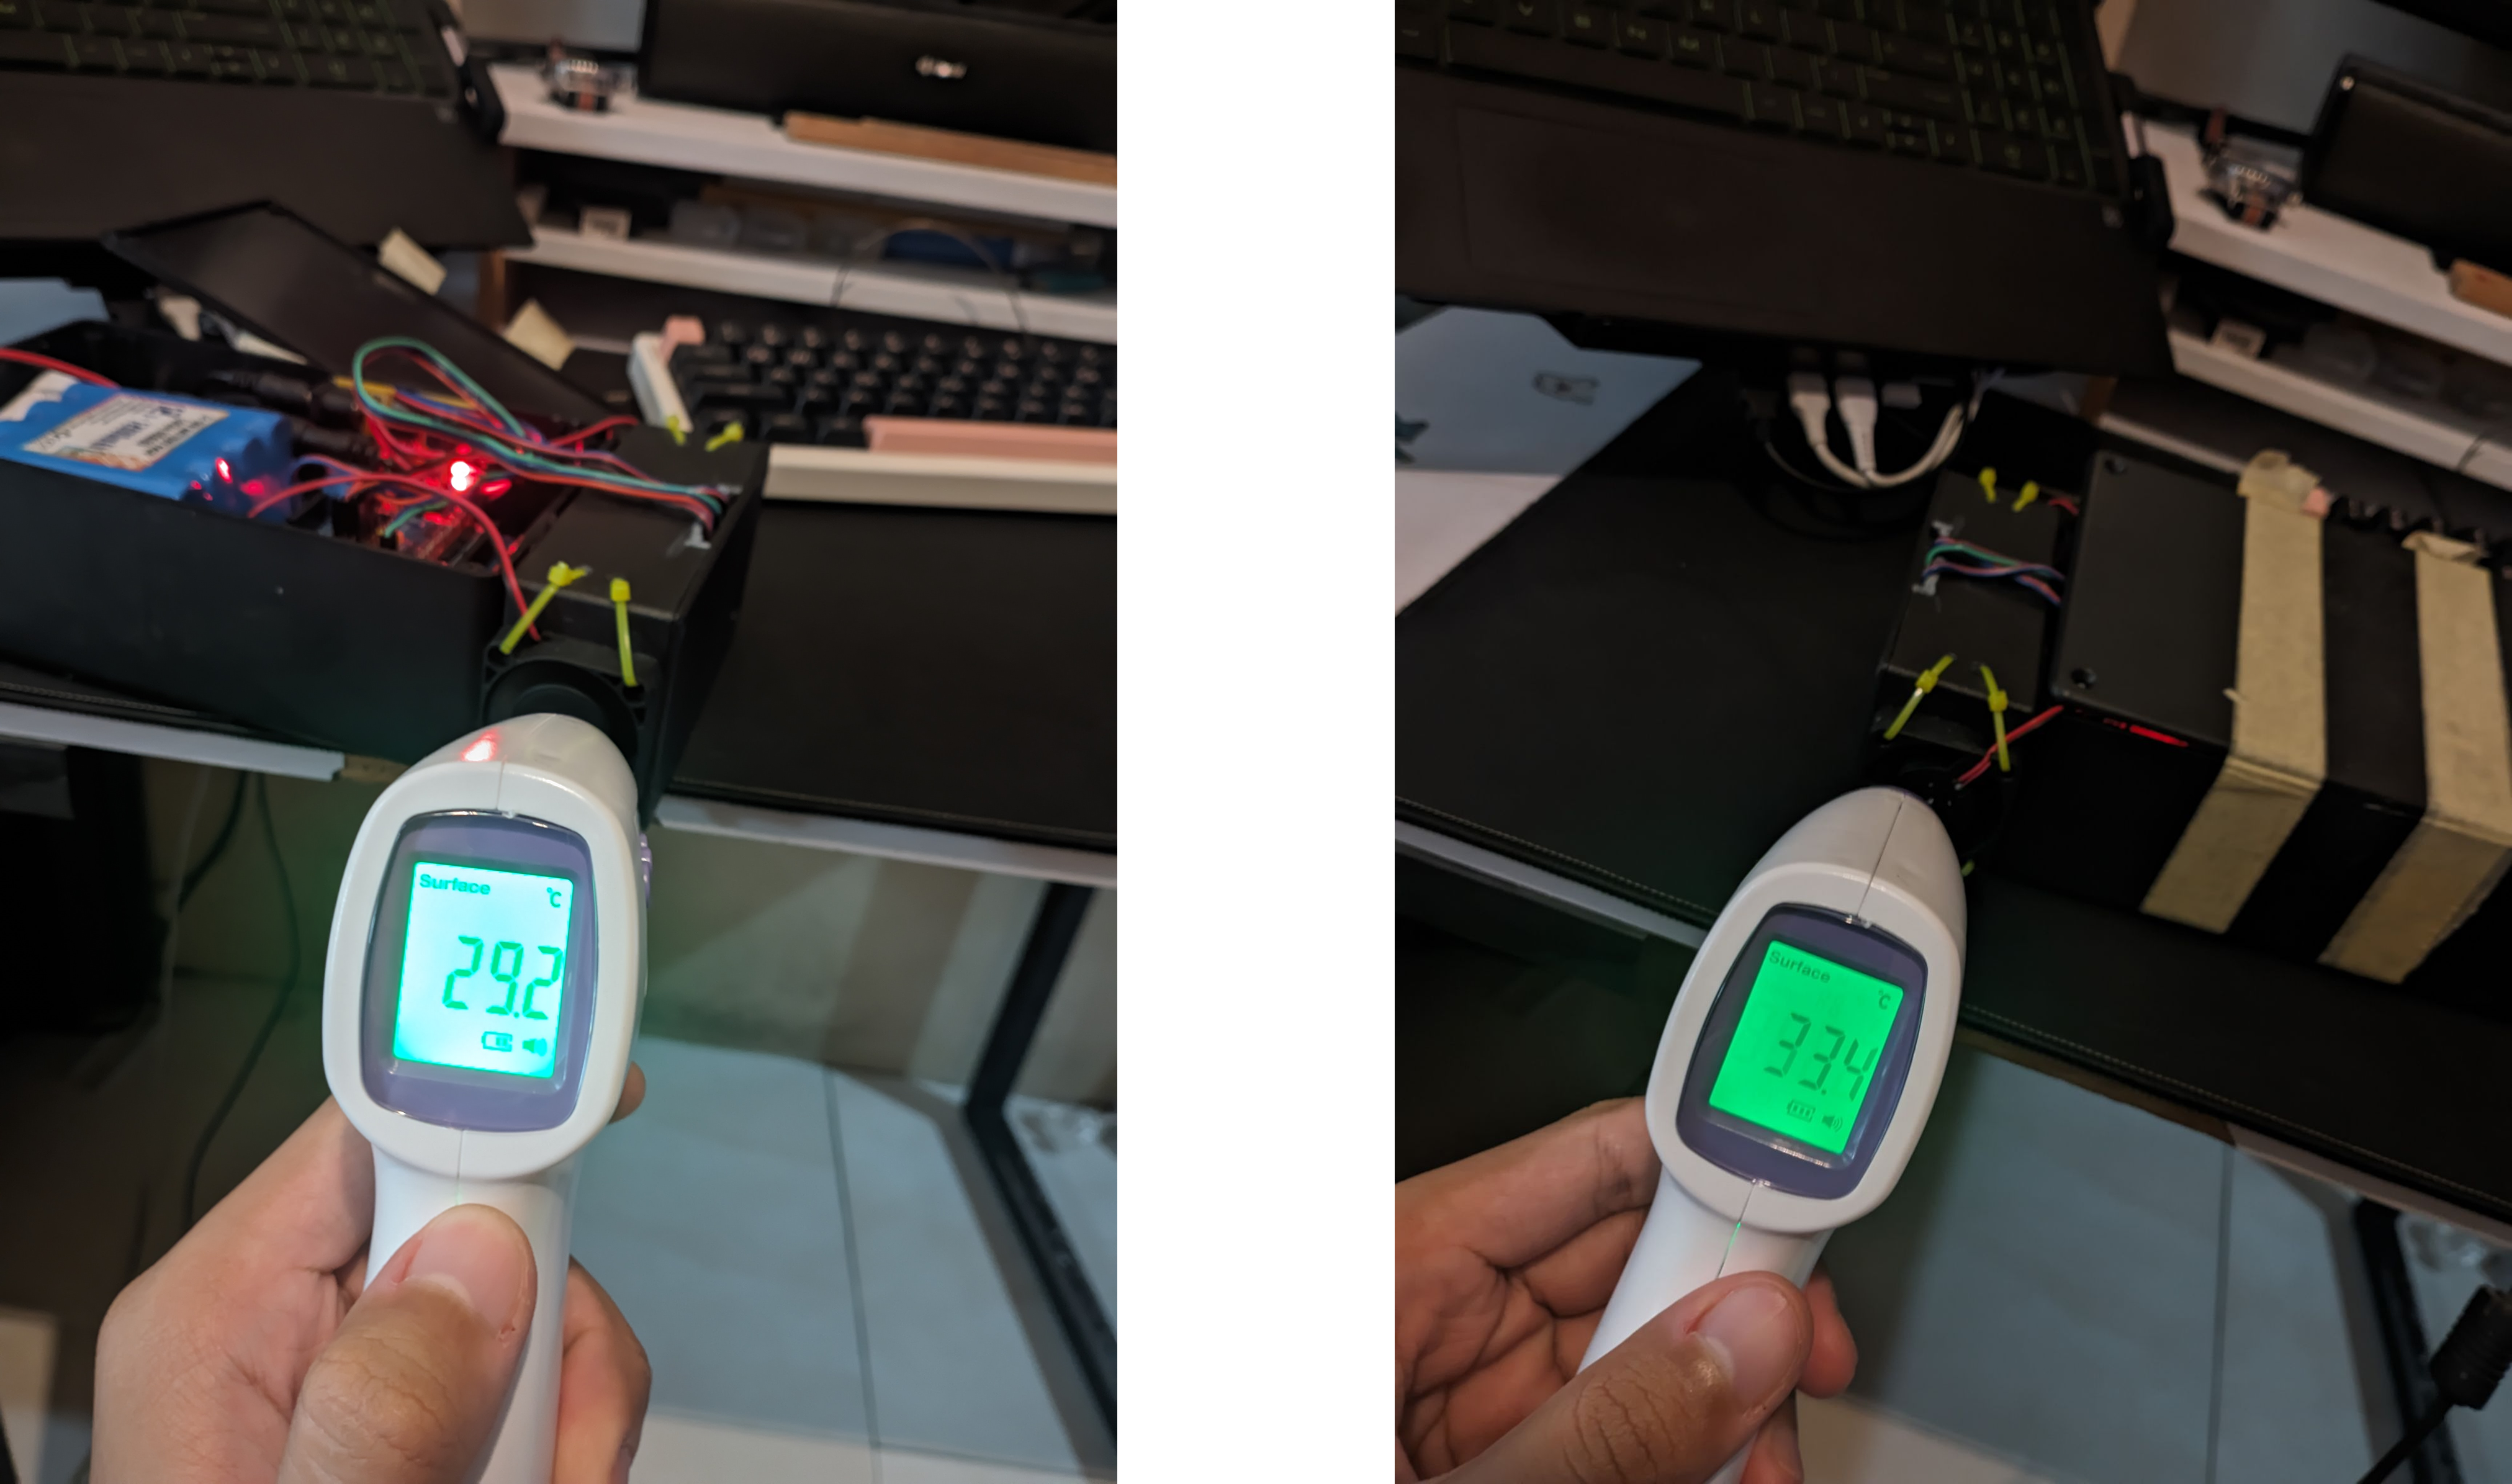
\includegraphics[width=\textwidth]{assets/pics/inout_indoor.png}
    \caption{Hasil Pembacaraan Thermometer Pada Kipas Intake (Kiri) dan Exhaust (Kanan) pada Suhu Ruangan}
    \label{fig:inout_indoor}
\end{figure}

Pada pengetesan \textit{indoor}, \textit{thermometer} membaca suhu pada kipas \textit{intake} berada pada angka $29.2^{\circ}$C dan \textit{exhaust} berada pada angka $33.4^{\circ}$C. Hal tersebut membuktikan bahwa dalam kondisi ruangan, sistem IoT masih dapat berjalan dengan ideal dan sensor-sensor masih bisa beroperasi dengan normal karena suhu ruangan \textit{mixing chamber} masih belum mendekati $50^{\circ}$C yang merupakan batasan suhu operasional setiap sensor. Berdasarkan pembacaan tersebut, kita dapat mengetahui rerata suhu pada \textit{mixing chamber} adalah $31.3^{\circ}$C.

\begin{figure}[t!]
    \centering
    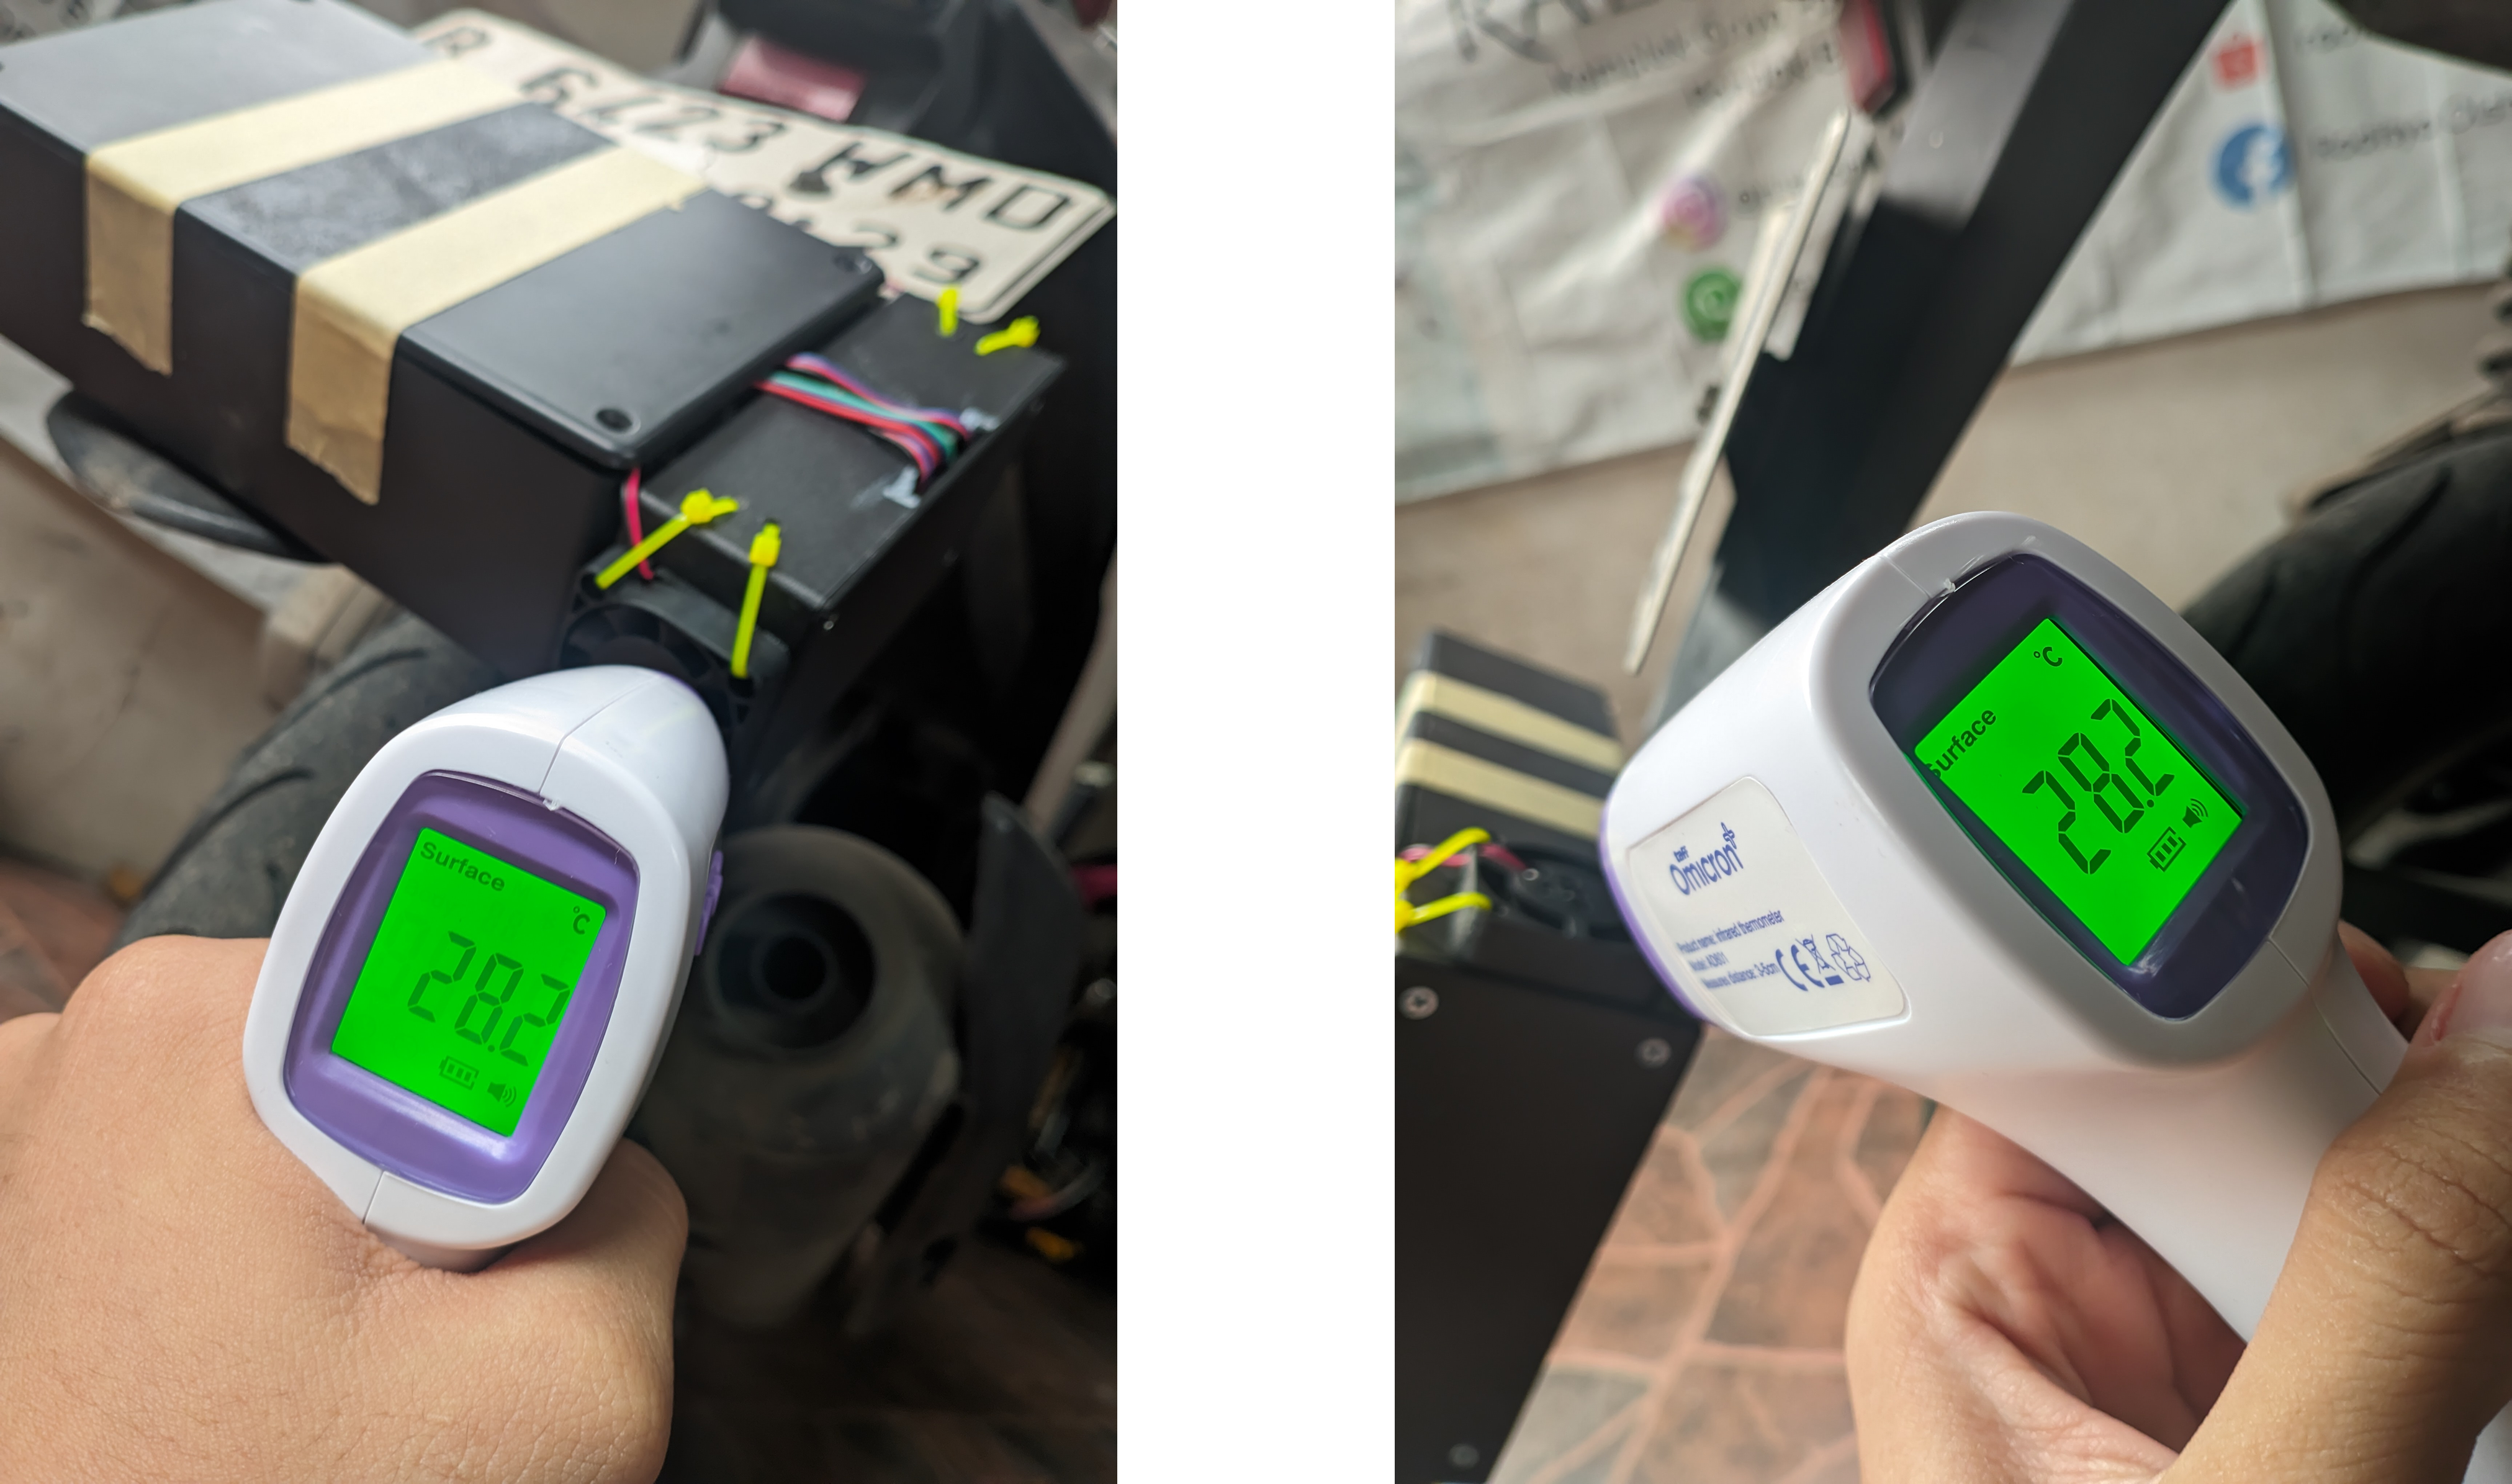
\includegraphics[width=\textwidth]{assets/pics/inout_pre_outdoor.png}
    \caption{Hasil Pembacaraan Thermometer Pada Kipas Intake (Kiri) dan Exhaust (Kanan) pada Sebelum Kendaraan Berjalan Bebas Selama 15 Menit}
    \label{fig:inout_pre_outdoor}
\end{figure}

Pada pengetesan \textit{outdoor}, \textit{thermometer} membaca suhu pada kipas \textit{intake} berada pada angka $28.2^{\circ}$C dan \textit{exhaust} berada pada angka $28.2^{\circ}$C. Hal tersebut membuktikan bahwa di luar ruangan ketika kendaraan bermotor belum dinyalakan, suhu pada area \textit{intake} dan \textit{exhaust} masih sama dengan kondisi suhu lingkungannya. Dan berdasarkan pembacaan tersebut kita dapat mengetahui rerata suhu pada \textit{mixing chamber} bernilai tetap, yaitu $28.2^{\circ}$C.

\begin{figure}[t!]
    \centering
    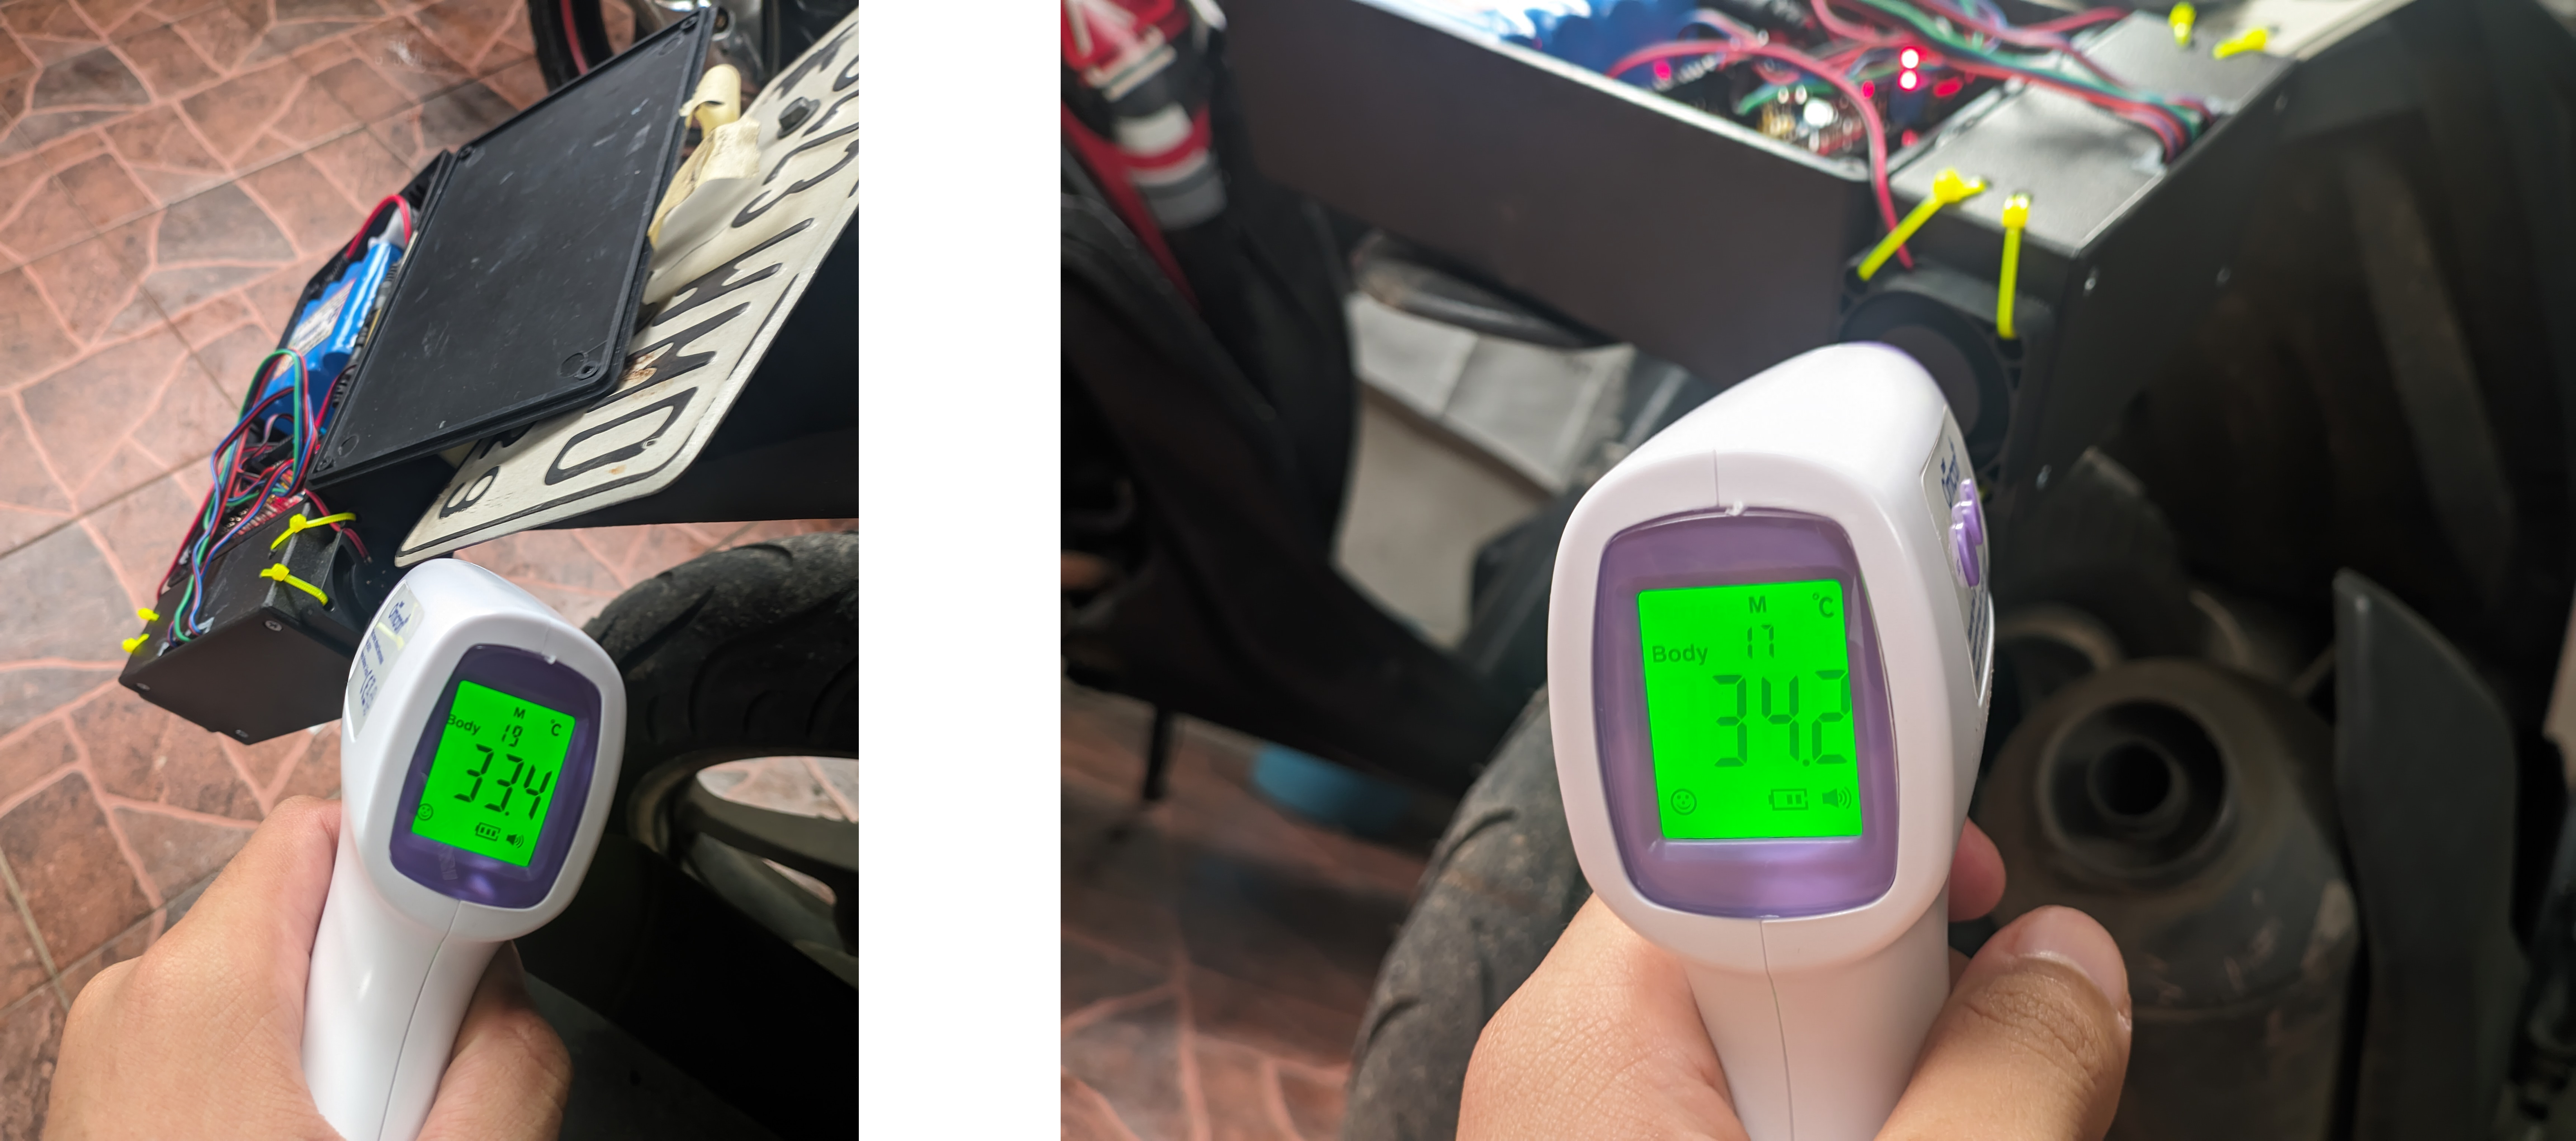
\includegraphics[width=\textwidth]{assets/pics/inout_post_outdoor.png}
    \caption{Hasil Pembacaraan Thermometer Pada Kipas Intake (Kiri) dan Exhaust (Kanan) pada Setelah Kendaraan Berjalan Bebas Selama 15 Menit}
    \label{fig:inout_post_outdoor}
\end{figure}

Setelah pengetesan \textit{outdoor} dilakukan, \textit{thermometer} membaca suhu pada kipas \textit{intake} berada pada angka 33.4$^{\circ}$C dan \textit{exhaust} berada pada angka 34.2$^{\circ}$C. Hal tersebut membuktikan bahwa di luar ruangan ketika kendaraan bermotor sudah dinyalakan dan berjalan secara bebas selama 15 menit, suhu pada area \textit{intake} dan \textit{exhaust} mengalami berubahan. Dan berdasarkan pembacaan tersebut kita dapat mengetahui rerata suhu pada \textit{mixing chamber} bernilai tetap, yaitu 33.8$^{\circ}$C.

Dengan adanya perubahan suhu baik pada kipas \textit{intake} maupun \textit{exhaust} ketika kendaraan dijalankan, menandakan bahwa sistem IoT yang dikembangkan berhasil mengalirkan aliran udara yang dihasilkan oleh saluran pembuangan hasil pembakaran kendaraan. Hasil yang didapat tersebut berhasil mengindikasikan bahwa suhu operasional sistem IoT pada \textit{Mixing Chamber} masih dalam kategori normal dan dapat ditoleransi oleh sensor-sensor yang di dalamnya.